\documentclass[conference]{IEEEtran}
\IEEEoverridecommandlockouts
% The preceding line is only needed to identify funding in the first footnote. If that is unneeded, please comment it out.
\usepackage{cite}
\usepackage{amsmath,amssymb,amsfonts}
\usepackage{algorithmic}
\usepackage{graphicx}
\usepackage{textcomp}
\usepackage{xcolor}
\usepackage{url}
\usepackage{listings}
\usepackage{graphicx} % Required for \resizebox
\usepackage{array} % Required for column width adjustments
\usepackage{tabularx}
\usepackage{balance}
\usepackage{colortbl} 
\usepackage{booktabs}
\usepackage{footnote}
\usepackage{multirow} 
 
\def\BibTeX{{\rm B\kern-.05em{\sc i\kern-.025em b}\kern-.08em
    T\kern-.1667em\lower.7ex\hbox{E}\kern-.125emX}}
\begin{document}

\title{Automating Maritime Risk Data \\Collection and Identification Leveraging \\Large Language Models}

% \title{1.Classification Model for Global Incidents and Establishing Data Collection Pipeline for Disaster Research. \\2.Automating Maritime Risk Data Collection and Categorization\\
% 3 Automating Maritime Risk Data Collection and Categorization: Comparing Traditional and Advanced Models}
% Which title is better? Can select and edit to produce a good title.
%We prefer the second one "Automating Maritime Risk Data Collection and Categorization" among the 3 possible title

\author{Anonymous Submission}

%\iffalse
\author{\IEEEauthorblockN{Donghao HUANG\textsuperscript{1,2},
 Xiuju FU\textsuperscript{3*}, Xiaofeng YIN\textsuperscript{3}, Haibo PEN\textsuperscript{4*}, Zhaoxia WANG\textsuperscript{1*}
}

\IEEEauthorblockA{School of Computing and Information Systems, Singapore Management University, Singapore\textsuperscript{1}}
\IEEEauthorblockA{Research and Development, Mastercard, Singapore\textsuperscript{2}}
\IEEEauthorblockA{Institute of High Performance Computing, Agency for Science, Technology and Research, Singapore\textsuperscript{3}}
\IEEEauthorblockA{School of Electrical and Information Engineering, Tianjin University, China\textsuperscript{4}}
\IEEEauthorblockA{dh.huang.2023@smu.edu.sg; fuxj@ihpc.a-star.edu.sg*; yinxf@ihpc.a-star.edu.sg; penhaibo@tju.edu.cn*; zxwang@smu.edu.sg*}
%\thanks{\IEEEauthorrefmark{1}
%Corresponding Authors: Zhaoxia WANG (e-mail: zxwang@smu.edu.sg)
%}
}
%\fi
\maketitle

\begin{abstract}
%This paper presents an innovative method for automating the collection and categorization of global maritime incident news, addressing limitations of traditional manual methods. We evaluate various classification models, including conventional machine learning approaches and advanced Large Language Models (LLMs) like GPT-4o and Llama-3.1. Our results demonstrate that LLMs, particularly GPT-4o, consistently outperform traditional models, significantly improving both efficiency and accuracy of maritime risk data collection. We introduce a new evaluation metric, the "Ratio of Valid Categories," to assess model reliability. Our findings contribute to the expanding literature on LLM applications in risk management, demonstrating their potential to transform data collection practices.
%zx-edit to focus on the contributions of this research

Maritime risk research is crucial yet challenging for improving safety, efficiency, and sustainability in maritime operations. This paper presents an innovative method for automating the collection and identification of risk data related to global maritime risks from news sources, addressing the limitations of traditional manual methods.
To evaluate the proposed method, different learning-based models, including conventional machine learning approaches and advanced Large Language Models (LLMs) such as GPT-4 and LLaMA-3.1, are comprehensively studied for comparison. 
In addition, not only do we use popular evaluation metrics to assess the proposed method, but we also introduce a new evaluation metric, called the "Ratio of Valid Categories ($RVC$)," to evaluate model reliability. The merits of the proposed method are demonstrated across different evaluation metrics.
The research results show that the proposed LLM-based methods, particularly the GPT-4-based method, consistently outperform traditional models, significantly improving both the efficiency and accuracy of maritime risk data collection and identification. Our findings contribute to the expanding literature on LLM applications in risk management, demonstrating their potential to transform data collection and identification practices.

\end{abstract}

\begin{IEEEkeywords}
%Maritime Risk Assessment, Automated Data Collection, Incident Categorization, Large Language Models, Few-shot Learning, Traditional Machine Learning, GPT-4o, Llama-3.1, Text Classification, Ratio of Valid Categories 
%zx edit to remove the keywords, which do not appear  in the abstract
Maritime Risk, Automated Data Collection, Risk Identification, Large Language Models, Traditional Machine Learning, GPT-4o, Llama-3.1, Ratio of Valid Categories ($RVC$) 
\end{IEEEkeywords}

% \begin{IEEEkeywords}
% Data Collection Pipeline, Maritime Risk Research, Incident Categorization, Large Language Models, Support Vector Machine, Naive Bayes, Random Forest, K-nearest Neighbors, Text Classification
% \end{IEEEkeywords}

\section{Introduction}
%\subsection{Background and Motivation}

The collection and analysis of risk or anomaly data from online news sources are critical for effective risk management~\cite{wang2013understanding, wang2014anomaly}. Maritime risk management and research are especially essential. However, traditional methods for gathering and categorizing such data are often labor-intensive, time-consuming, and expensive~\cite{babelsenticnet,blending,camsta,ngulea}. Existing approaches rely heavily on manual effort for data labeling and annotation, which not only incurs significant operational costs but also limits scalability. For instance, using services like NewsAPI for comprehensive data collection can be prohibitively expensive\footnote{News API Pricing: \url{https://newsapi.ai/plans}}, with search volumes insufficient to meet the needs of advanced risk information analytics.

Recent advancements in machine learning (ML) and natural language processing (NLP) have begun to address these challenges by automating parts of the data collection and classification pipeline~\cite{nlu,7pillars,hu2023msrl,primenet,wang2023learning, jiisui,hu2021stock}. 

Specifically:
\begin{itemize}
    \item Teske et al. proposed a two-step NLP pipeline using traditional ML models like Logistic Regression and AdaBoost to classify maritime incident articles and extract relevant information\cite{teske2018automatic}.
    
    \item Jidkov et al. further enhanced this approach using deep learning techniques such as convolutional neural networks (CNNs) to identify specific types of incidents, although their models faced challenges like overfitting due to limited training data\cite{jidkov2020enabling}.
    
    \item Subsequent research by Mackenzie et al.  introduced advanced metadata extraction techniques using models like CatBoost to improve the accuracy of information retrieval from unstructured news articles\cite{mackenzie2021maritime}.
\end{itemize}

While these traditional ML and deep learning models have shown promise, they are often limited by the quality and volume of labeled data available for training. The emergence of Large Language Models (LLMs) like GPT-3 and its successors has marked a significant shift in NLP capabilities. LLMs such as OpenAI's GPT-4o can perform a wide range of NLP tasks, including text classification, summarization, and entity extraction, using few-shot learning---a technique that requires only a few examples to achieve high performance. Brown et al. demonstrated that scaling up language models improves their adaptability to new and diverse input data, which is crucial for maritime risk assessment models where real-time data is heterogeneous and constantly evolving\cite{brown2020language}.

Building on these advancements, this paper presents a novel pipeline that leverages LLMs to automate the collection and categorization of global incident news. Our approach integrates traditional ML models and state-of-the-art LLMs, such as GPT-4o, to evaluate their effectiveness in news classification tasks. We find that LLMs, particularly GPT-4o, consistently outperform traditional models, enhancing both the efficiency and accuracy of maritime risk data collection. The proposed pipeline not only streamlines the categorization process but also ensures the timely delivery of relevant insights, which is vital for proactive risk management.\\

This study contributes to the growing body of literature on the application of LLMs in risk management by demonstrating their superiority over traditional models in handling complex, real-world datasets. We also introduce a new evaluation metric, the ``Ratio of Valid Categories,'' to measure the reliability of model outputs in classification tasks. This metric provides deeper insights into the performance of various models, highlighting the importance of model robustness and data quality in automated data collection pipelines.

%\subsection{Contributions}
Our main contributions are:
\begin{itemize}
    \item Develop a new method for automated maritime risk data collection and identification.
    \item Propose a new evaluation metric: Ratio of Valid Categories ($RVC$).
    \item Analyze and compare the capabilities of the proposed method with traditional ML models and LLMs for maritime risk identification from news.
    \item Demonstrate the merits of the proposed method with LLMs in maritime risk data collection and identification across different evaluation methods.
\end{itemize}

% \section{Introduction}
% \subsection{Background and Motivation}

% The collection and analysis of maritime risk data from online news sources are critical for effective risk management and research. However, traditional methods for gathering and categorizing such data are often labor-intensive, time-consuming, and expensive. Existing approaches rely heavily on manual effort for data labeling and annotation, which not only incurs significant operational costs but also limits scalability. For instance, using services like NewsAPI for comprehensive data collection can be prohibitively expensive\footnote{News API Pricing: \url{https://newsapi.ai/plans}}, with search volumes insufficient to meet the needs of advanced risk information analytics.

% Recent advancements in machine learning (ML) and natural language processing (NLP) have begun to address these challenges by automating parts of the data collection and classification pipeline. Teske et al. proposed a two-step NLP pipeline using traditional ML models like Logistic Regression and AdaBoost to classify maritime incident articles and extract relevant information. Jidkov et al.  further enhanced this approach using deep learning techniques such as convolutional neural networks (CNNs) to identify specific types of incidents, although their models faced challenges like overfitting due to limited training data. Subsequent research by Mackenzie et al.  introduced advanced metadata extraction techniques using models like CatBoost to improve the accuracy of information retrieval from unstructured news articles.

% While these traditional ML and deep learning models have shown promise, they are often limited by the quality and volume of labeled data available for training. The emergence of Large Language Models (LLMs) like GPT-3 and its successors has marked a significant shift in NLP capabilities. LLMs such as OpenAI’s GPT-4o can perform a wide range of NLP tasks, including text classification, summarization, and entity extraction, using few-shot learning—a technique that requires only a few examples to achieve high performance. Brown et al.  demonstrated that scaling up language models improves their adaptability to new and diverse input data, which is crucial for maritime risk assessment models where real-time data is heterogeneous and constantly evolving.

% Building on these advancements, this paper presents a novel pipeline that leverages LLMs to automate the collection and categorization of global incident news. Our approach integrates traditional ML models and state-of-the-art LLMs, such as GPT-4o, to evaluate their effectiveness in news classification tasks. We find that LLMs, particularly GPT-4o, consistently outperform traditional models, enhancing both the efficiency and accuracy of maritime risk data collection. The proposed pipeline not only streamlines the categorization process but also ensures the timely delivery of relevant insights, which is vital for proactive risk management.

% This study contributes to the growing body of literature on the application of LLMs in risk management by demonstrating their superiority over traditional models in handling complex, real-world datasets. We also introduce a new evaluation metric, the "Ratio of Valid Categories," to measure the reliability of model outputs in classification tasks. This metric provides deeper insights into the performance of various models, highlighting the importance of model robustness and data quality in automated data collection pipelines.

% In summary, our work aims to enhance the efficiency of maritime risk management by automating data collection and categorization processes using advanced NLP models. The findings underscore the potential of LLMs to transform risk assessment practices, reducing the need for manual labor and improving the accuracy and reliability of incident data analysis.

% \subsection{Contributions}
% Our main contributions are:
% \begin{itemize}
%     \item Development of an automated pipeline for maritime risk data collection and categorization
%     \item Comparative analysis of traditional ML models and LLMs in maritime news classification
%     \item Introduction of a new metric: Ratio of Valid Categories (RVC)
%     \item Demonstration of LLMs' superior performance in maritime risk data processing
% \end{itemize}




% The task of collecting online news reports for event monitoring often involves time-intensive processes, leading researchers to spend a disproportionate amount of time on data management rather than on critical analysis. A study conducted in 2020 by Spasic et al\cite{spasic2020clinical}. highlighted that, while using text data to classify clinical narratives, data collection emerged as the most significant challenge. The researchers found that extensive manual labor was required, resulting in poor data utilization, where only a portion of the collected data could be effectively used for machine learning models. Additionally, the process of labeling and annotating text data demands substantial human effort, with annotators meticulously tagging each document with relevant metadata. Although this human-driven approach ensures high-quality labeled data, it also imposes significant operational overhead and hinders the scalability of data collection efforts. 
% For example, using services like newsapi.ai for comprehensive data collection can be prohibitively expensive. While 200,000 searches per month cost around \$1,300\footnote{News API Pricing: \url{https://newsapi.ai/plans}}, this search volume is insufficient for conducting advanced risk information analytics.
% This highlights the significant financial and labor-related costs associated with traditional news data collection methods.

% Given these challenges, there is a clear need for innovative approaches to incident monitoring and risk management and research, particularly those that can streamline the data collection process. Advances in Large Language Models (LLMs) present an opportunity to develop more efficient classification models and data collection pipelines, enabling researchers to better harness the vast amount of information available in the digital space. This paper focuses on improving the data collection process for news articles, specifically those related to incidents and disasters worldwide. We will explore the design, implementation, and evaluation of traditional classification models and the recent breakthroughs in Large Language Models, comparing their performance in news classification tasks. Our goal is to provide insights into optimizing these systems to support in-depth research and analysis in risk management and studies.

\section{Related Work}

\subsection{Traditional Machine Learning Approaches}

Before the emergence of large language models (LLMs), traditional machine learning approaches, such as Support Vector Machines (SVM), Na\"ive Bayes (NB), and k-Nearest Neighbors (KNN), were widely utilized for text classification tasks~\cite{chalea}. Luo conducted a comprehensive analysis of these methods, demonstrating that SVM consistently outperformed other classifiers, such as Na\"ive Bayes and Logistic Regression, in terms of classification accuracy for English text documents~\cite{luo2021efficient}. The study highlighted the effectiveness of SVM, achieving classification rates exceeding 90\% when using more than 4,000 features, while the Rocchio classifier yielded the best results for smaller feature sets.

\subsection{Large Language Models and Their Impact}

The advent of large language models (LLMs) has significantly transformed natural language processing methodologies. Brown et al. introduced GPT-3, a 175-billion-parameter autoregressive language model capable of performing various NLP tasks, such as translation, question-answering, and text completion, with strong performance in a few-shot learning setting, where the model is prompted with only a few examples instead of requiring task-specific fine-tuning~\cite{brown2020language}. This few-shot capability is particularly valuable in domains like maritime risk assessment, where adaptability to new and diverse input data is essential. Brown et al.'s study underscores that scaling up language models can lead to significant improvements in few-shot learning, which can be leveraged to enhance the classification and extraction of incident information in specialized datasets.

\subsection{Expanding Capabilities of LLMs}

Further evaluations have demonstrated the expanding capabilities of LLMs across various domains:

\begin{itemize}
    \item \textbf{Affective Computing:} Amin et al. (2023) evaluated the performance of ChatGPT models, including GPT-3.5, on affective computing tasks such as suicide tendency detection, personality assessment, and sentiment analysis~\cite{senticnet}, confirming the emerging capabilities of ChatGPT in these areas~\cite{amin2023will}. The study found that while ChatGPT models performed comparably to classical NLP methods like Bag-of-Words and Word2Vec, they still lagged behind fine-tuned language models such as RoBERTa for specific tasks.

    \item \textbf{Text Summarization:} Basyal and Sanghvi (2023) investigated the capabilities of LLMs in text summarization, conducting a comparative study across different LLMs. Their findings demonstrated that models like OpenAI's text-davinci-003 significantly outperformed others in generating concise summaries, as indicated by higher BLEU, ROUGE, and BERT scores~\cite{basyal2023text}.

    \item \textbf{Text Classification:} Chae and Davidson (2023) conducted a comprehensive study on the application of LLMs for text classification, from zero-shot learning to fine-tuning approaches~\cite{chae2023large}. Their research demonstrated how different LLM architectures, including GPT variants, perform in text classification tasks, highlighting their ability to generalize with minimal training examples. The study indicated that while larger models, such as GPT-3 and GPT-4, achieve higher accuracy, smaller models fine-tuned on specific datasets can also perform competitively at a fraction of the cost, making them an attractive option for many research applications. It further discussed the trade-offs between proprietary and open-source models, emphasizing the importance of evaluating models for bias and transparency.

    \item \textbf{Retrieval Augmented Generation (RAG):} Recent studies have explored the use of LLMs in Retrieval Augmented Generation (RAG) and in-context learning tasks. Huang and Wang (2024) evaluated Microsoft's Orca 2 in RAG applications, comparing it with models like GPT-4 and GPT-3.5-Turbo~\cite{huang2024evaluation}. Their study found that Orca 2 excelled in generating high-quality responses efficiently on consumer-grade GPUs. Similarly, Huang et al. (2024) assessed Llama 2's performance in in-context learning using the MS MARCO dataset~\cite{huang2024performance}. The results showed that Llama-2 models performed comparably to OpenAI's offerings, with Llama-2-13b-chat-hf slightly outperforming GPT-3.5-turbo in answer quality.
\end{itemize}

\section{Dataset}

The dataset used in this study, named the \textit{Global Maritime Risk Incident Dataset (GMRID)}, consists of an extensive collection of global maritime risk data, with a primary focus on incidents and disasters. The original dataset contains 5,744 records, each characterized by 52 distinct attributes. A detailed examination revealed that most of these attributes were manually appended after the initial data collection process. This manual enrichment indicates that the core dataset initially consisted of two fundamental attributes: \textit{Category} and \textit{Details}.

%To automate the data collection process, a classification model is necessary to accurately label each maritime disruption according to its risk category.

Before applying the dataset to classification models, several preprocessing steps were undertaken to enhance the quality of the text data in the \textit{Details} column. These steps included converting text to lowercase, tokenizing, removing punctuation, eliminating stopwords, and lemmatizing words. Such preprocessing was essential to standardize the data and reduce noise, thereby improving model performance.

The dataset includes a \textit{Category} column summarizing the types of disruptions; however, this column was initially unstructured, containing 857 unique labels. To address this issue, the \textit{Category} column was split using a comma delimiter, resulting in 111 unique labels. Recognizing that this number remained too large for effective classification, further consolidation reduced the number of labels to eight primary categories. Table~\ref{tab:event_categories} presents the mapping between the eight primary categories and the initial unstructured categories. This mapping is performed by four human annotators, who are researchers involved in this study.

During our experiments, we observed significant discrepancies between the labels generated through the manual process described above and those produced by the \textit{gpt-4o} model. A manual review of these discrepancies showed a preference for the \textit{gpt-4o} model's labeling in 9 out of 10 cases (refer to Table \ref{tab:comparison_results} in Section \ref{subsec:v1_vs_v2}). As a result, we opted to use the \textit{gpt-4o} model with a 5-shot prompting strategy to relabel all entries in the dataset. The revised dataset is referred to as \textit{GMRID v2}, while the original dataset is referred to as \textit{GMRID v1}.

%zx better showcase the difference between v1 and V2

\begin{table*}[ht]
\caption{Mapping of Initial Unstructured Categories to Eight Primary Categories for Maritime Risk Classification. This table illustrates the consolidation of 857 unique labels into 8 primary categories, demonstrating the process of data refinement for more effective classification. The mapping was performed by four human annotators involved in the study.}
% , showcasing the manual effort required in preparing the dataset for automated classification tasks.}
\centering
\small
\setlength{\tabcolsep}{4pt}
\renewcommand{\arraystretch}{1.13}
\resizebox{.7\textwidth}{!}{
\begin{tabularx}{\textwidth}{|>{\raggedright\arraybackslash\hspace{0pt}}p{2.3cm}|>{\raggedright\arraybackslash\hspace{0pt}}X|}
\hline
\textbf{Primary Categories} & \textbf{Initial Unstructured Categories} \\
\hline
Weather & Flooding, Severe Winds, Weather Advisory, Tropical Cyclone, Storm, Ice Storm, Earthquake, Tornado, Typhoon, Landslide, Water, Hurricane, Wildfire, Blizzard, Hail \\
\hline
Worker Strike & Mine Workers Strike, Production Halt, Protest, Riot, Port Strike, General Strike, Civil Service Strike, Civil Unrest Advisory, Cargo Transportation Strike, Energy Sector Strike \\
\hline
Administrative Issue & Port Congestion, Police Operations, Roadway Closure, Disruption, Cargo, Industrial Action, Port Disruption, Cargo Disruption, Power Outage, Port Closure, Maritime Advisory, Train Delays, Ground Transportation Advisory, Public Transportation Disruption, Trade Regulation, Customs Regulation, Regulatory Advisory, Industry Directives, Security Advisory, Public Holidays, Customs Delay, Public Health Advisory, Detention, Aviation Advisory, Waterway Closure, Plant Closure, Border Closure, Delay, Industrial Zone Shutdown, Trade Restrictions, Closure, Truck Driving Ban, Insolvency, Environmental Regulations, Postal Disruption, Travel Warning \\
\hline
Human Error & Workplace Accident, Individuals in Focus, Military Operations, Flight Delays, Cancellations, Political Info, Political Event \\
\hline
Cyber Attack & Network Disruption, Ransomware, Data Breach, Phishing \\
\hline
Terrorism & Bombing, Warehouse Theft, Public Safety, Security, Organized Crime, Piracy, Kidnap, Shooting, Robbery, Cargo Theft, Bomb Detonation, Terror Attack, Outbreak Of War, Militant Action \\
\hline
Accident & Hazmat Response, Maritime Accident, Vehicle Accident, Death, Injury, Non-industrial Fire, Chemical Spill, Industrial Fire, Fuel Disruption, Airline Incident, Crash, Explosion, Train Accident, Derailment, Sewage Disruption, Barge Accident, Bridge Collapse, Structure Collapse, Airport Accident, Force Majeure, Telecom Outage \\
\hline
Others & Miscellaneous Events, Miscellaneous Strikes, Outbreak of Disease \\
\hline
\end{tabularx}
}
\label{tab:event_categories}
\end{table*}


% To streamline our analysis and enhance the relevance of our findings, we selected eight attributes that most effectively represent the dataset. These attributes were organized into four categories to facilitate a more structured examination, as illustrated in Table \ref{tab:attributes_table}.

% \begin{table*}[ht!]
% \centering
% \resizebox{\textwidth}{!}{
% \begin{tabular}{|p{0.2\textwidth}|p{0.75\textwidth}|}
% \hline
% \textbf{Attributes} & \textbf{Explanation and Example} \\ \hline
% \multicolumn{2}{|l|}{\textbf{1. News Attributes}} \\ \hline
% Headline & The headline of the news, for example: \\
% & \textit{“Access road to Yantian container terminals closed from November 24-26”} \\ \hline
% Details & Summary of the news, this attribute details the causation of the incident, specific location, and time of the event, for example: \\
% & \textit{“Local sources report on November 23 that due to roadwork on the Wutong Bridge, a key access road to A gate to the Yantian container terminals will be closed from November 24 at 00:00 to November 26 at 08:00 local time. This will likely cause delays in pick-up and deliveries of containers to the port as drivers will need to divert to gate B to enter the port.”} \\ \hline
% \multicolumn{2}{|l|}{\textbf{2. Important Categorical Attributes}} \\ \hline
% Severity & Attributes that categorize the incidents' severity into four levels: \\
% & \textit{‘minor’, ‘moderate’, ‘severe’, and ‘extreme’} \\ \hline
% Region & Values are the countries where incidents occurred, for example: \\
% & \textit{“China”, “United States”, “Australia”, etc.} \\ \hline
% Category & The attributes are the type of the incident or disaster, for example: \\
% & \textit{‘Trade restriction’, ‘Travel Warning’, ‘Port Congestion’, etc.} \\ \hline
% \multicolumn{2}{|l|}{\textbf{3. Geographical Attributes}} \\ \hline
% Lat (Latitude) & \textit{“29.52”, “29.86875”} \\ \hline
% Log (Longitude) & \textit{“121.3319”, “31.03305”} \\ \hline
% \multicolumn{2}{|l|}{\textbf{4. Time Series Attributes}} \\ \hline
% Datetime & In the format of Day/Month/Year Hour:Minute \\
% & \textit{“7/1/19 9:50”, “27/4/19 15:46”} \\ \hline
% \end{tabular}
% }
% \caption{Overview of Selected Attributes and Their Explanations}
% \label{tab:attributes_table}
% \end{table*}

% \subsection{Exploratory Data Analysis}

% Our analysis of over 5,000 recorded incidents reveals that China, the United States, and Australia report the highest number of cases (Figure~\ref{fig:top_regions}). Notably, 497 of these incidents were categorized as severe or extreme (Figure~\ref{fig:event_severity}), indicating their significant economic impact or substantial loss of life.

% \begin{figure*}[ht]
%     \centering
%     \includegraphics[width=0.9\textwidth]{figures/top_regions.png}
%     \caption{Geographic Distribution of Reported Incidents}
%     \label{fig:top_regions}
% \end{figure*}

% \begin{figure}[ht]
%     \centering
%     \includegraphics[width=\columnwidth]{figures/event_severity.png}
%     \caption{Distribution of Incident Severity Across All Cases}
%     \label{fig:event_severity}
% \end{figure}


\section{Methodology}

%\subsection{Operational Pipeline for News Data Collection}
\subsection{Overview of the Proposed Method}

The proposed method is designed to streamline the risk data collection and identification from news sources for users. This section details the proposed method as an operational pipeline from the perspective of a user using the system.

The proposed method, as illustrated in Fig.~\ref{fig:pipeline}, automates the summarization, identification, and updating of disruption database based on the URLs submitted by users. The process is designed to be intuitive and user-friendly, allowing users to efficiently collect and analyze the risk data.

\begin{figure*}[ht!]
\centering
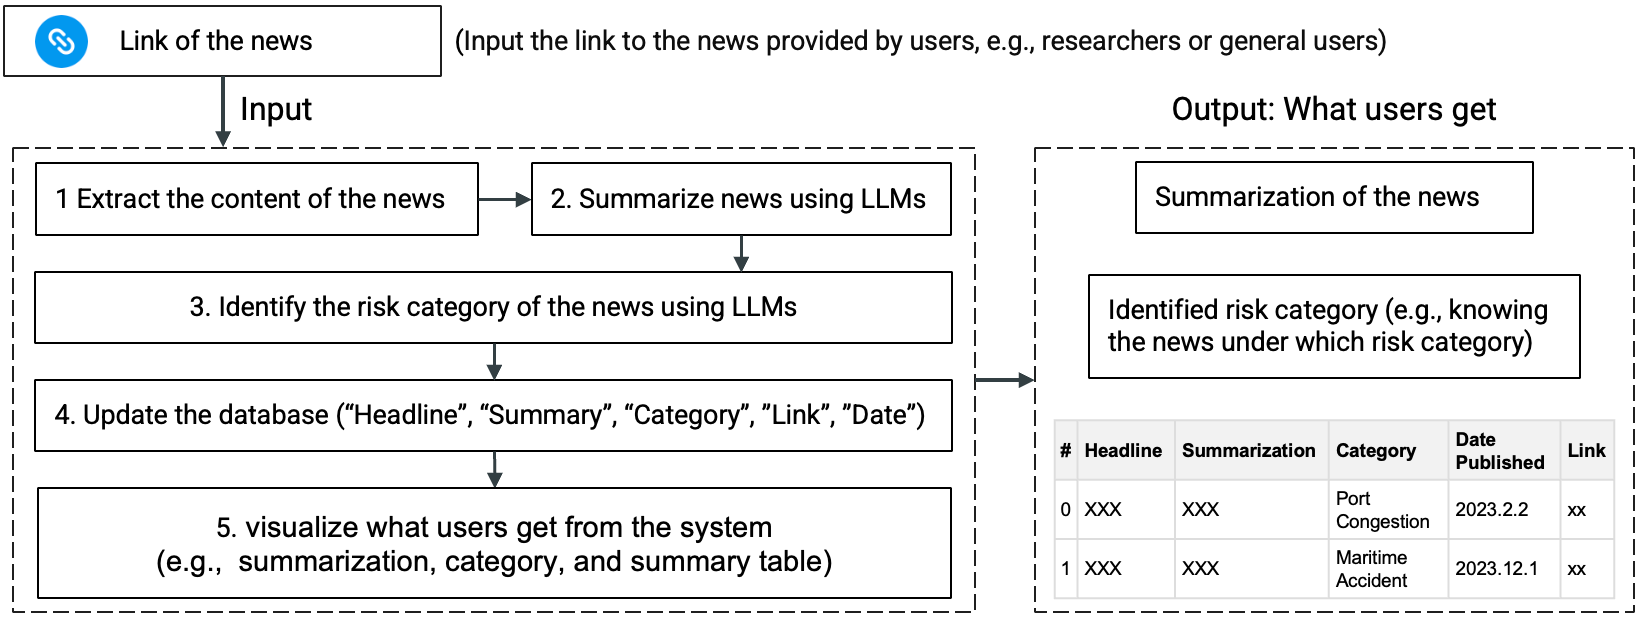
\includegraphics[width=0.66\textwidth]{figures/pipeline.png}
\caption{Schematic Overview of the Proposed Method: Operational Pipeline for Risk Data Collection and Identification from News Sources. This figure illustrates the step-by-step process of the automated risk data collection and identification system, from URL submission by users to the generation of a summary table. Key steps include: 1. Extract the content of the news, 2.Summarize the news using LLMs, 3. Identify the risk category of the news using LLMs, 4. Update the database, and 5. Visualize what users get from the system. 
%The pipeline demonstrates the integration of LLM capabilities with traditional database operations to streamline maritime risk data analysis.
}
\label{fig:pipeline}
\end{figure*}


As shown in Fig.~\ref{fig:pipeline}, the interaction begins when a user submits the URL of a disruption event. In the first key step (Step 1), the system extracts the content of the news and checks whether the event already exists in the database. If the event is new, the model will proceed with the following steps: summarizing the news, identifying the risk category, updating the database with the key elements, and presenting a summary of the information to users through visualization. This summary provides users with a quick overview of the news article’s content.
The prompt used for summarizing by LLM is shown in Listing \ref{lst:summary-prompt}.

\vspace{1.5\baselineskip}
\begin{lstlisting}[caption={Prompt for LLM Summarization}, 
                   label={lst:summary-prompt}, 
                   breaklines=true, 
                   basicstyle=\footnotesize\ttfamily, 
                   xleftmargin=0pt, 
                   framexleftmargin=0pt, 
                   framesep=0pt, 
                   aboveskip=0pt, 
                   belowskip=0pt, 
                   showspaces=false, 
                   showstringspaces=false,
                   keepspaces=true,
                   breakindent=0pt]
Summarize the following article in about 70 words, focusing on what happened, where it happened, and the consequences (economic loss, environmental impact, etc.): {article}
\end{lstlisting}

Following the summarization (Step 2: Summarize the news using LLMs), the model identifies the risk category (Step 3: Identify the risk category of the news using LLMs). The results from both steps are used in the subsequent step to better organize the data into meaningful segments, enhancing usability for users. For this research, we evaluated the performance of traditional ML models and modern Large Language Models (GPT-4, Llama-3.1). Our comparative analysis focused on key performance metrics, such as accuracy and the ability to discern nuanced distinctions across diverse news topics.

Once the identification (Step 3) is complete, Step 4: Update the database will be conducted. This step involves updating and enriching the database by adding detailed records, including the event's headline, summary, risk category, URL link, and publication date. To further support user-friendly efforts, the model identifies and ranks related news events within the same category based on their recency. This functionality enables users to quickly access the most current and relevant information within their area of interest.

For enhanced risk data presentation, the system is designed to visualize what users get from it (Step 5). The system not only visualizes the summarization of the news and the identified risk category but also generates a summary table that distills the collected data into an easy-to-digest format, presenting key information such as headlines, summaries, categories, and publication dates. 
%For instance, if a user is analyzing the impact of earthquakes, they can discover recent earthquake events and explore related articles. The model retrieves related articles categorized under 'earthquake,' prioritizing those with greater recency. This ensures that users have access to the most up-to-date and contextually relevant information, as older articles may not reflect current economic conditions, building standards, or environmental policies.

\subsection{Comparative Study of GMRID Identification: Traditional Models vs. LLMs}

In this study, we evaluated the performance of both traditional classification models and modern Large Language Models (LLMs) such as GPT-4o and Llama-3.1. Our comparative analysis focused on key performance metrics, including accuracy and the ability to distinguish nuanced differences across diverse news topics.

We implemented five traditional machine learning models---Naive Bayes, Logistic Regression, Support Vector Machine (SVM), Random Forest, and K-Nearest Neighbors---using the scikit-learn library\footnote{\url{https://scikit-learn.org/}}. Training, evaluation, and hyper-parameter tuning were conducted with both the GMRID v1 and v2 datasets.

In addition to traditional models, we employed OpenAI’s GPT-4o and GPT-4o-mini, as well as Meta's Llama-3.1-8B and Llama-3.1-70B models, for classification tasks. The dataset was split into two subsets, with 80\% used for training and 20\% reserved for testing.

To enable the LLMs to perform classification, we utilized few-shot prompting techniques. The system prompt template used for this classification is provided in Listing \ref{lst:llm-classification-prompt}.

\vspace{2.0\baselineskip}
\begin{lstlisting}[caption={Prompt for LLM Classification}, 
                   label={lst:llm-classification-prompt}, 
                   breaklines=true, 
                   basicstyle=\scriptsize\ttfamily, 
                   xleftmargin=0pt, 
                   framexleftmargin=0pt, 
                   framesep=0pt, 
                   aboveskip=0pt, 
                   belowskip=0pt, 
                   showspaces=false, 
                   showstringspaces=false,
                   keepspaces=true,
                   breakindent=0pt]
Task: You are a classifier. Your objective is to analyze the given input and assign it to one of the predefined categories: {categories}. Evaluate the content carefully and use the defining characteristics of each category to ensure an accurate classification.

Guidelines:
1. Understand the Categories: Familiarize yourself with the specific attributes of each category by referring to the category descriptions provided in the JSON: {categories_json}.
2. Contextual Analysis: Consider the broader context of the input. If an input could potentially fit into multiple categories, select the one that best reflects its primary intent or focus.
3. Handling Ambiguity: For ambiguous inputs or those that do not clearly align with any category, choose the category that most closely matches the content provided.
4. Ensure Accuracy and Consistency: Strive for consistent and accurate classifications. Avoid arbitrary or random assignments.
5. Provide Feedback: If the input cannot be classified into any of the given categories, return "Others".
{exemplars}
Output Format: Return only the name of the category that the input belongs to. If uncertain, respond with "Others".
\end{lstlisting}

The system prompt template is designed as a versatile tool for text classification. In our study, the placeholders were populated with the following specific data:

\begin{itemize}
    \item \texttt{\{categories\}}: A list of primary categories, as shown in Table \ref{tab:event_categories}.
    \item \texttt{\{categories\_json\}}: A JSON structure mapping primary categories to initial unstructured categories, as detailed in Table \ref{tab:event_categories}.
    \item \texttt{\{exemplars\}}: For zero-shot classification, this field is left empty; for few-shot classification, exemplars are retrieved from the GMRID training set and formatted as shown in Listing \ref{lst:exemplars-prompt}.
\end{itemize}

\begin{lstlisting}[caption={Exemplars Used in Few-Shot Prompting}, 
                   label={lst:exemplars-prompt}, 
                   breaklines=true, 
                   basicstyle=\scriptsize\ttfamily, 
                   xleftmargin=0pt, 
                   framexleftmargin=0pt, 
                   framesep=0pt, 
                   aboveskip=0pt, 
                   belowskip=0pt, 
                   showspaces=false, 
                   showstringspaces=false,
                   keepspaces=true,
                   breakindent=0pt]
Example Inputs and Outputs:
- Input: local source reported operation at pier 1 and 2 of the container terminal at port of durban was suspended due to strong winds ...
- Classification: Weather
... 
\end{lstlisting}

%the Port of Durban was suspended due to strong winds on December 27 at 18:50 local time, resuming at 23:10 the same day. Pier 2 terminal operations were halted at 19:30 and resumed at 20:35 respectively.

Using the above prompting techniques, the evaluation of GPT-4o and GPT-4o-mini models was conducted via the OpenAI API\footnote{\url{https://platform.openai.com/docs/overview}}, while the evaluation of Llama-3.1 models was performed on Nvidia L40 GPUs using the HuggingFace Transformers library\footnote{\url{https://huggingface.co/docs/transformers/en/index}}.

\subsection{Evaluation Metrics}

To evaluate the performance of each model, we calculated predictive accuracy on the held-out test data using the weighted F1 score. This metric provides an overall measure of the model’s performance by taking into account both precision and recall, giving a balanced view of the model's ability to correctly classify data.

During the evaluation process, we observed that the Large Language Models (LLMs) occasionally produced outputs that did not correspond to any valid category labels defined in Table \ref{tab:event_categories}. Table \ref{tab:classification_results} presents a sample of classification results produced by the Llama-3.1-8B model, using different numbers of shots (0, 1, 3, 5, and 10).

\begin{table}[ht]
\caption{Sample Classification Results from Llama-3.1-8B Model Using Different Numbers of Shots. This table presents the outputs of the Llama-3.1-8B model for a single input across varying numbers of shots (0, 1, 3, 5, and 10). It illustrates the model's tendency to produce lengthy explanations and justifications, particularly with fewer shots, highlighting the challenge of generating concise, valid category labels consistently.}
\centering
\setlength{\tabcolsep}{6pt} % Adjust column padding
\renewcommand{\arraystretch}{1.2} % Adjust row height
\begin{tabularx}{.49\textwidth}{|>{\raggedright\arraybackslash\hspace{0pt}}p{1.2cm}|>{\raggedright\arraybackslash\hspace{0pt}}X|}
\hline
\textbf{Details (Cleaned)} & thursday reported operation u.s. air cargo company like fedex ups affected novel coronavirus covid-19 quarantine testing measure imposed 
official china report chinese official told flight crew would required quarantine ... \\
\hline
\textbf{Ground Truth} & Administrative Issue \\
\hline
\textbf{0-shot(s) Result} & Based on the provided input, the category that best fits the content is 'Administrative Issue'. The input discusses ... \\
\hline
\textbf{1-shot(s) Result} & Based on the provided input, the classification is: Others. \textit{Reasoning}: The input discusses the impact of COVID-19 quarantine measures on air cargo operations in China ... \\
\hline
\textbf{3-shot(s) Result} & Based on the input, the classification is: Administrative Issue. \\
\hline
\textbf{5-shot(s) Result} & Based on the input, the classification is: Administrative Issue. \\
\hline
\textbf{10-shot(s) Result} & Administrative Issue \\
\hline
\end{tabularx}
\label{tab:classification_results}
\end{table}

Based on the results in Table \ref{tab:classification_results}, we observe that the Llama-3.1-8B model correctly classifies the input as 'Administrative Issue' when given 10 shots. However, in other cases, the model produces lengthy explanations and justifications for its classifications, resulting in outputs that do not directly align with the predefined categories. These outputs are deemed "invalid categories" and cannot be directly used for performance calculations. To address this issue, we developed a post-processing function to extract valid categories from the LLM outputs, ensuring accurate computation of the F1 scores.

We also noted that "invalid categories" were more frequent in the smaller models, which often lack the capability to strictly follow instructions, undermining the reliability of their performance in classification tasks.

To further quantify this issue, we introduced a new metric called the Ratio of Valid Categories ($RVC$):

\begin{equation}
\text{$RVC$} = \frac{\text{Number of Valid Categories}}{\text{Total Number of Entries}}
\end{equation}

A “valid category” is any output generated by the model that matches the predefined set of category labels. 
This metric, $RVC$, provides insight into each model's reliability in producing valid classifications. A higher ratio indicates greater consistency in assigning entries to valid categories, which is crucial in classification tasks where the accuracy of labels directly affects the model's effectiveness.


\section{Results and Discussions}

\subsection{Performance Evaluation: GMRID v1 vs. v2}
\label{subsec:v1_vs_v2}

We conducted classification using various machine learning models, including OpenAI's models with few-shot prompting, to determine their optimal performance settings. The best results of this evaluation are presented in Table \ref{tab:classification_model_evaluation_v2}.

\begin{table}[ht]
\caption{Classification Model Evaluation - Results Comparison Between GMRID v1 (Annotator-Labeled Ground Truth) and GMRID v2 (GPT-4o Labeled Ground Truth). This table presents the F1 scores of various machine learning models, including traditional approaches and LLMs, on both datasets. It demonstrates the performance improvement observed when using the GPT-4o labeled dataset (v2) compared to the human-labeled dataset (v1), suggesting potential benefits of LLM-generated ground truth for training and evaluation.}
\centering
\renewcommand{\arraystretch}{1.2}
\resizebox{0.4\textwidth}{!}{
\begin{tabular}{|c|c|c|}
\hline
\textbf{Model}          & \textbf{F1 Score (GMRID v1)} & \textbf{F1 Score (GMRID v2)} \\ \hline
Naive Bayes             & 79.93\%                      & 87.61\%                      \\ \hline
Logistic Regression     & 80.39\%                      & \textbf{90.74\%}            \\ \hline
Support Vector Machine  & \textbf{81.63\%}             & 90.08\%                      \\ \hline
Random Forest           & 80.73\%                      & 87.80\%                      \\ \hline
K-nearest Neighbors     & 79.81\%                      & 83.32\%                      \\ \hline
\midrule % Separates the groups
GPT-4o-mini             & 62.85\% (3-shot)             & 93.86\% (1-shot)             \\ \hline
GPT-4o                  & \textbf{65.06\%} (5-shot)             & \textbf{98.76\%} (5-shot)             \\ \hline
\end{tabular}
}
\label{tab:classification_model_evaluation_v2}
\end{table}

The lower performance of the OpenAI models on the GMRID v1 dataset warrants further investigation. To gain a deeper understanding of this issue, we conducted a manual inspection of the results from the top-performing run: \textit{gpt-4o} with 5-shot prompting. Our analysis revealed that, in most instances where the model's output differed from the human-labeled ground truth, the model's classification appeared to be more accurate. Table~\ref{tab:comparison_results} presents a comparison of 10 such cases, where \textit{gpt-4o} provided a more accurate label in 9 out of 10 instances.

\begin{table*}[ht]
\caption{Comparative Analysis of Original Human-Annotated Labels and GPT-4o Generated Labels for Maritime Risk Classification. This table presents 10 sample cases where the GPT-4o model's classification differed from the original human-labeled ground truth. Bolded entries denote the label deemed more accurate after manual review, with GPT-4o being favored in 9 out of 10 cases.}
\centering
\small
\setlength{\tabcolsep}{4pt}
\renewcommand{\arraystretch}{1.2}
\resizebox{0.8\textwidth}{!}{
\begin{tabularx}{\textwidth}{|>{\raggedright\arraybackslash}X|>{\raggedright\arraybackslash}p{2.3cm}|>{\raggedright\arraybackslash}p{2.3cm}|}
\hline
\textbf{Details (Cleaned)} & \textbf{Original Label} & \textbf{GPT-4o Generated Label} \\
\hline
port captaincy cartagena dimar declared second time hotel la américas responsible for undue occupation of beach mangrove area; hotel owner comment. & Others & \textbf{Administrative Issue} \\
\hline
government source indicates casualties due to nationwide flooding in kenya. flooding caused by heavy rain impacting horn of africa. government coordinating with kenyan red cross and ngos. & Terrorism & \textbf{Weather} \\
\hline
fire in coal harbour impacted an underground homeless encampment. skytrain service disruptions, evacuation due to smoke. fire controlled, ongoing rail disruption. & Administrative Issue & \textbf{Accident} \\
\hline
three people killed due to poisoning/suffocation in a ship cabin belonging to new energy engineering company.% ltd., shanghai. 
& Terrorism & \textbf{Accident} \\
\hline
china gearing up for chinese new year; factory shutdowns and shipping disruptions expected. higher freight costs anticipated due to increased demand before the holiday. & Worker Strike & \textbf{Administrative Issue} \\
\hline
explosion and fire aboard a vessel at charleston harbor marina; three injured. emergency services on site. & Terrorism & \textbf{Accident} \\
\hline
tropical storm narda caused port closure in manzanillo, mexico; operations resumed. %on september 30. 
& Administrative Issue & \textbf{Weather} \\
\hline
caledonian sleeper service canceled due to planned industrial action by rmt union members. %from september 29 to october 1. 
& Administrative Issue & \textbf{Worker Strike} \\
\hline
8 individuals arrested in new jersey for a multi-million-dollar cargo theft ring. stolen goods included various products from warehouses. & \textbf{Administrative Issue} & Terrorism \\
\hline
heavy rain and strong winds forecasted to hamper operations at the port of colombo. & Administrative Issue & \textbf{Weather} \\
\hline
\end{tabularx}
}
\label{tab:comparison_results}
\end{table*}

The results in Table \ref{tab:classification_model_evaluation_v2} highlight several key observations. Firstly, the v2 dataset, where labels were generated by the \textit{gpt-4o} model, shows improved accuracy for nearly all machine learning models, suggesting that the generated labels are more consistent or better suited to the patterns these models learn.

Furthermore, the OpenAI models, particularly \textit{gpt-4o} with a 5-shot strategy, significantly outperform traditional machine learning models on the v2 dataset, achieving the highest accuracy of 98.76\%. This demonstrates the potential of few-shot prompting with advanced models like \textit{gpt-4o} to deliver superior results, particularly when the ground truth is generated by a similar model.

The noticeable performance differences between the v1 and v2 datasets for the same models suggest potential biases or inconsistencies in human-labeled data that may not align with the patterns these models learn. Consequently, using models like \textit{gpt-4o} for generating ground truth labels could provide a more consistent foundation for training and evaluating classification models.

Overall, these findings suggest that integrating advanced language models with few-shot learning strategies can significantly enhance classification performance, especially when the ground truth data is generated or verified by the same type of models.


\subsection{LLM Classification Performance: Open Source vs. Proprietary Models}

We evaluated the performance of the Llama-3.1 models (8B and 70B) using few-shot prompting and compared their performance against the OpenAI models (GPT-4o and GPT-4o-mini) using the GMRID v2 dataset. Table~\ref{tab:llm_comparison} presents the F1 scores and the ratio of valid categories across different numbers of shots (0, 1, 3, 5, and 10) for each model.

\begin{table}[ht]
\caption{Comprehensive Performance Comparison of Llama-3.1 Models (8B and 70B) and OpenAI Models (GPT-4o-mini and GPT-4o) Across Different Few-Shot Prompting Scenarios. This table presents both F1 scores and Ratio of Valid Categories (RVC) for each model under varying numbers of shots. The the best performance for each model highlighted in bold.}
\centering
\renewcommand{\arraystretch}{1.2}
\resizebox{.45\textwidth}{!}{
\begin{tabular}{|l|c|c|c|c|c|c|}
\hline
\textbf{Model} & \textbf{Metric} & \textbf{0-shot} & \textbf{1-shot} & \textbf{3-shot} & \textbf{5-shot} & \textbf{10-shot} \\ \hline
\multirow{2}{*}{Llama-3.1-8B} & F1  & 71.51\% & \textbf{87.08\%} & 86.52\% & 86.35\% & 77.28\% \\
 & RVC & 49.43\% & 91.28\% & 92.94\% & 92.68\% & \textbf{99.13}\% \\ \hline
\multirow{2}{*}{Llama-3.1-70B} & F1  & 92.54\% & 93.20\% & 93.83\% & 93.95\% & \textbf{94.01\%} \\
 & RVC & 99.56\% & 99.91\% & \textbf{100.00\%} & \textbf{100.00\%} & \textbf{100.00\%} \\ \hline
\multirow{2}{*}{gpt-4o-mini} & F1  & 92.18\% & \textbf{93.86\%} & 91.92\% & 92.54\% & 92.97\% \\
 & RVC & 99.91\% & \textbf{100.00\%} & \textbf{100.00\%} & 99.91\% & 99.74\% \\ \hline
\multirow{2}{*}{gpt-4o} & F1  & 94.97\% & 97.42\% & 97.46\% & \textbf{98.76\%} & 97.12\% \\
 & RVC & \textbf{100.00\%} & \textbf{100.00\%} & \textbf{100.00\%} & \textbf{100.00\%} & \textbf{100.00\%} \\ \hline
\end{tabular}
}
\label{tab:llm_comparison}
\end{table}

The results reveal several key insights:

\begin{itemize}
    \item \textbf{GPT-4o}: Consistently achieves the highest F1 scores across all numbers of shots, with a peak performance of 98.76\% at 5-shot. It also maintains a perfect 100\% ratio of valid categories across all scenarios, demonstrating the highest level of robustness and reliability among the models tested.
    
    \item \textbf{Llama-3.1-70B}: Shows competitive performance, particularly in maintaining valid categories. It achieves 100\% validity from 3-shot onwards, matching GPT-4o in this aspect. Its F1 scores, while lower than GPT-4o, are consistently above 90\%, peaking at 94.01\% for 10-shot.
    
    \item \textbf{GPT-4o-mini}: Performs well overall but shows minor inconsistencies, particularly in the ratio of valid categories at 0-shot (99.91\%), 5-shot (99.91\%), and 10-shot (99.74\%). Its F1 scores are generally lower than GPT-4o but competitive with Llama-3.1-70B.

    \item \textbf{Llama-3.1-8B}: This model exhibits the highest variability in performance. It demonstrates a substantial improvement in the ratio of valid categories, increasing from 49.43\% at 0-shot to 99.13\% at 10-shot. However, despite the enhancement in F1 scores with additional shots, its performance remains inferior to that of other models. The F1 score peaks at 87.08\% for 1-shot, which is notably lower than the performance of most traditional machine learning models presented in Table~\ref{tab:classification_model_evaluation_v2}. This discrepancy underscores the challenges faced by smaller language models in achieving consistent performance across various few-shot configurations.
\end{itemize}

These findings highlight the impact of model size and architecture on classification performance in few-shot learning contexts. While the proprietary GPT-4o model maintains superior performance across all metrics, the larger Llama-3.1-70B model demonstrates competitive results, particularly in maintaining valid categories. This suggests that open-source models are closing the gap with proprietary ones, especially in terms of output consistency. The performance variations across different shot numbers also underscore the importance of selecting appropriate few-shot prompts for optimal model performance.



\balance
\section{Conclusion and Future Work}

This study presents a novel approach for automating the collection and categorization of global maritime disruption data, utilizing the capabilities of Large Language Models (LLMs) like GPT-4o. The findings reveal that LLMs, particularly GPT-4o, significantly outperform traditional machine learning models in terms of both accuracy and consistency, proving to be more effective in classifying complex news data. The introduction of the "Ratio of Valid Categories" metric provided valuable insights into the reliability of each model, with GPT-4o achieving a perfect 100\% ratio of valid categories across all scenarios. Although other models, such as GPT-4o-mini and Meta-Llama-3.1, demonstrated some variability, the results underscore the potential of LLMs in enhancing risk data collection and research capabilities. The findings also emphasize the importance of selecting robust models and highlight the role of LLMs in streamlining data-driven risk management.

While the results of this study are promising, several limitations must be acknowledged. The primary limitation is the quality of the available data, which inherently contains ambiguities and inconsistencies due to the diverse nature of news articles. These characteristics pose significant challenges for accurate categorization.
Moreover, the use of GPT-4o for relabelling the data may introduce biases, particularly as the model is also evaluated on this dataset. To mitigate these potential biases and to ensure more robust validation, future work will incorporate comprehensive human evaluation.
% Future research will aim to address these limitations by improving data quality and refining evaluation methodologies. There is considerable scope for exploring more advanced LLM models, including fine-tuning LLMs to enhance classification accuracy further. Continued research in these areas will be crucial for advancing the field of automated maritime risk management.
Moving forward, research will focus on improving data quality and refining evaluation methodologies. Exploring more advanced LLM models and fine-tuning them for better classification accuracy will be critical for advancing automated maritime risk management.

\section*{Acknowledgment}

The authors express their sincere appreciation to the students from Singapore Management University (SMU) for their enthusiastic interest and invaluable contributions to this paper: LU Quanfang, WEI Yifan, YANG Xinyue, and LIAO Jiaxiong. Their dedication has significantly enriched our research. This work was supported by the Natural Science Foundation
of Tianjin under Grant 19JCQNJC06000.

\bibliographystyle{IEEEtran}
\bibliography{references}

\end{document}
